\label{chap:building_corpus}

Since we wanted the translation memory to be functional from the very beginning, we needed to build a parallel corpus -- preferably from some repository of subtitles.

Right after we received the data from \emph{opensubtitles.org} and had the ``raw'' subtitle data, we started to build a parallel corpus from this data to use it for the translation memory. The process of creating the corpus and getting the ``clean'' translation memory data is described in the following sections.

Since there were more strategies how to process the ``raw'' data which looked equally promising, we also needed to develop a measure of the quality of the resulting corpus (either by measuring the alignment itself or the resulting corpus).

In this chapter, we discuss these steps, together with a more detailed description of the data we received. We will also discuss various strategies for measuring the quality of the corpus.

\section{Retrieving Data}

There are hundreds to thousands of subtitle files in any major language available on the Internet, and all of those can be easily downloaded individually, file by file. However, for building a bigger corpus, we need the biggest number of subtitles possible -- and it is problematic to download from most of the servers in bigger batches (due to the anti-robot protection and so on).

Also, since we wanted to avoid any copyright problems, we would meet by using random subtitles, randomly downloaded from the Internet. Because of that, we directly asked the administrator of the biggest server providing the subtitle site \url{http://www.opensubtitles.org} for the data. We will refer to the website as OS.org in the following chapters.

We were extremely lucky to receive all subtitle files in Czech and English (but only from media sources, that have subtitles from both of these languages) from OS.org with following license condition (in Slovak):

\begin{quote}
\begin{verbatim}
Titulky mozem poskytnut, s tym ze:

- nebudu sa dalej sirit
- vsade, kde je to mozne a suvisi to s projektom, bude uvedena linka na
    www.opensubtitles.org (stranka programu, dokumentacia, program...)

Co sa tyka autorskych prav, tak neviem presne ako to je, ale myslim,
ze to je +- ok :)
\end{verbatim}
\end{quote}

\noindent -- English translation:

\begin{quote}
\begin{verbatim}
We can provide the subtitle files under following conditions:

- they won't be provided any further
- a link to www.opensubtitles.org will be placed whenever it's possible 
   (web page of the program, documentation, program itself...)

Considering the copyright law, I am not really sure how it is, 
but I think it's ok :)
\end{verbatim}
\end{quote}


\noindent We decided that this license condition is acceptable for our purposes. 

%As a matter of fact, 
The contents of OS.org is all user-generated, and users of OS.org, when uploading files, agree with a statement where they declare they are holders of all rights to the content they upload, and that they provide the subtitle files as their own intellectual property for public use. Based on this and the license, we think there are no copyright issues.% Based on this statement we trust the users they really did what they declared.

%From this data we will create a parallel corpus of ...

\section{The Initial Data Properties}
\label{sec:properties}
\subsubsection*{Format}
The OpenSubtitles data consisted of the following files:
\begin{itemize}
    \item file, called \texttt{export.txt.gz}, which was a tab-separated table, having information about one subtitle file on one line. The information consisted of:
    \begin{itemize}
        \item ID of a media source (an internal OS.org ID)
        \item name of the subtitle file (a number)
        \item language of the subtitle (either czech or english)
        \item ID of the subtitle (in the case of split subtitles, the ID is the same, while name of the file is different)
        \item information on how many parts the movie was split and which part this subtitles belong to
        \item format of the subtitle (\emph{always} \texttt{srt})
        \item description of media source. This description consists of the name of the movie in the case of movies, or of the name of the series and episode in the case of TV shows. What is also present is the year of the movie release.
        
         We found out these data are taken from IMDB (internally, by OS.org) and in almost all the cases determine the movie unambiguously. There are very few cases of two movies with the same name released in the same year, and the probability of both of them having both Czech and English translation is low. We took the name and the year as unambiguously identifying a media source.
    \end{itemize}
    
    There were 676,155 lines in the document (which would imply 676 155 files). There is 15,882 separate media sources in the file (which would imply 42.6 files for one document).
    \item 139,538 gzipped subtitle files (filenames as described in the table + \texttt{.gz})
\end{itemize}
All these files were packed into a \texttt{tar} file, with a size of 3,076 MB.

\subsubsection*{Cleaning up -- non-existent files}
As you can see even just by looking at the numbers, the data in the database and the files do not match up exactly. So the initial clean-up was getting only the intersection of files we have and the files that are in the database. 

The intersection is 39,712 Czech subtitle files and 97,991 English files of 15,881 media sources -- 3,032 MB of zipped data.

\subsubsection*{Cleaning up -- split subtitles}
The other step in cleanup is -- for simplicity -- removing the subtitles that are split to multiple files; we assumed that those split into more parts are probably just split version the complete ones. 81\,\% of subtitles are in one piece and only 1.7\,\% movies have subtitles only in multiple files. By deleting subtitles split into more files, we completely lose the Czech side of 64 movies and English the side of 218 movies, which is 3,5\% in total.

\subsubsection*{Cleaning up -- Carmencita}
There was also one peculiar issue with the media sources. While looking more carefully at the data, we found there were 228 Czech subtitles files, 814 files in total having one particular movie ID and containing absolutely different content. This movie was Carmencita, a 21 seconds long silent film from 1894\footnote{See \url{http://en.wikipedia.org/wiki/File:Carmencita.ogg} for details.}. We concluded this very probably happened due to a server error at OS.org, because the movie has the ID {\tt tt0000001} at IMDB. We deleted those as well.

%Because OpenSubtitles internally uses IMDB for adding information about movies and TV shows to subtitles, it was not hard to align subtitles of same movies and TV show episodes together, since all movie names used the same format (name and year), and the TV episodes were all correctly marked.

\subsubsection*{Cleaning up -- results}
After performing all the mentioned filtering, we had 2,543 MB in 110,312 gzipped subtitle files (32,705 Czech, 77,607 English) of 15,552 movies / TV shows' episodes.

When we did a simple check to find out, how many subtitles are actually in \texttt{srt} format we found out, that from 110,312 subtitles, 432 are not regular \texttt{srt} and might actually be \texttt{sub} (but sometimes, they are, for example, HTML files, or just strange binary data). That means that only 0.39\% of subtitle files are not \texttt{srt}. We are noting it here, because we later based some of our decision based on this

All previous cleanup was done as one of the first things when we received the data; it is not included in the \emph{dataimport} module and the module already expects these data filtered out.

Later in development, we noticed that some files have incorrect language written in the table file; files, that should be in Czech, were in  Hungarian, and so on. We added language detection, based on letter trigrams, later; that detection is, however, already in the \emph{dataimport} module and is done directly before aligning the files (which will be described later).


\begin{figure}[t]
\begin{center}
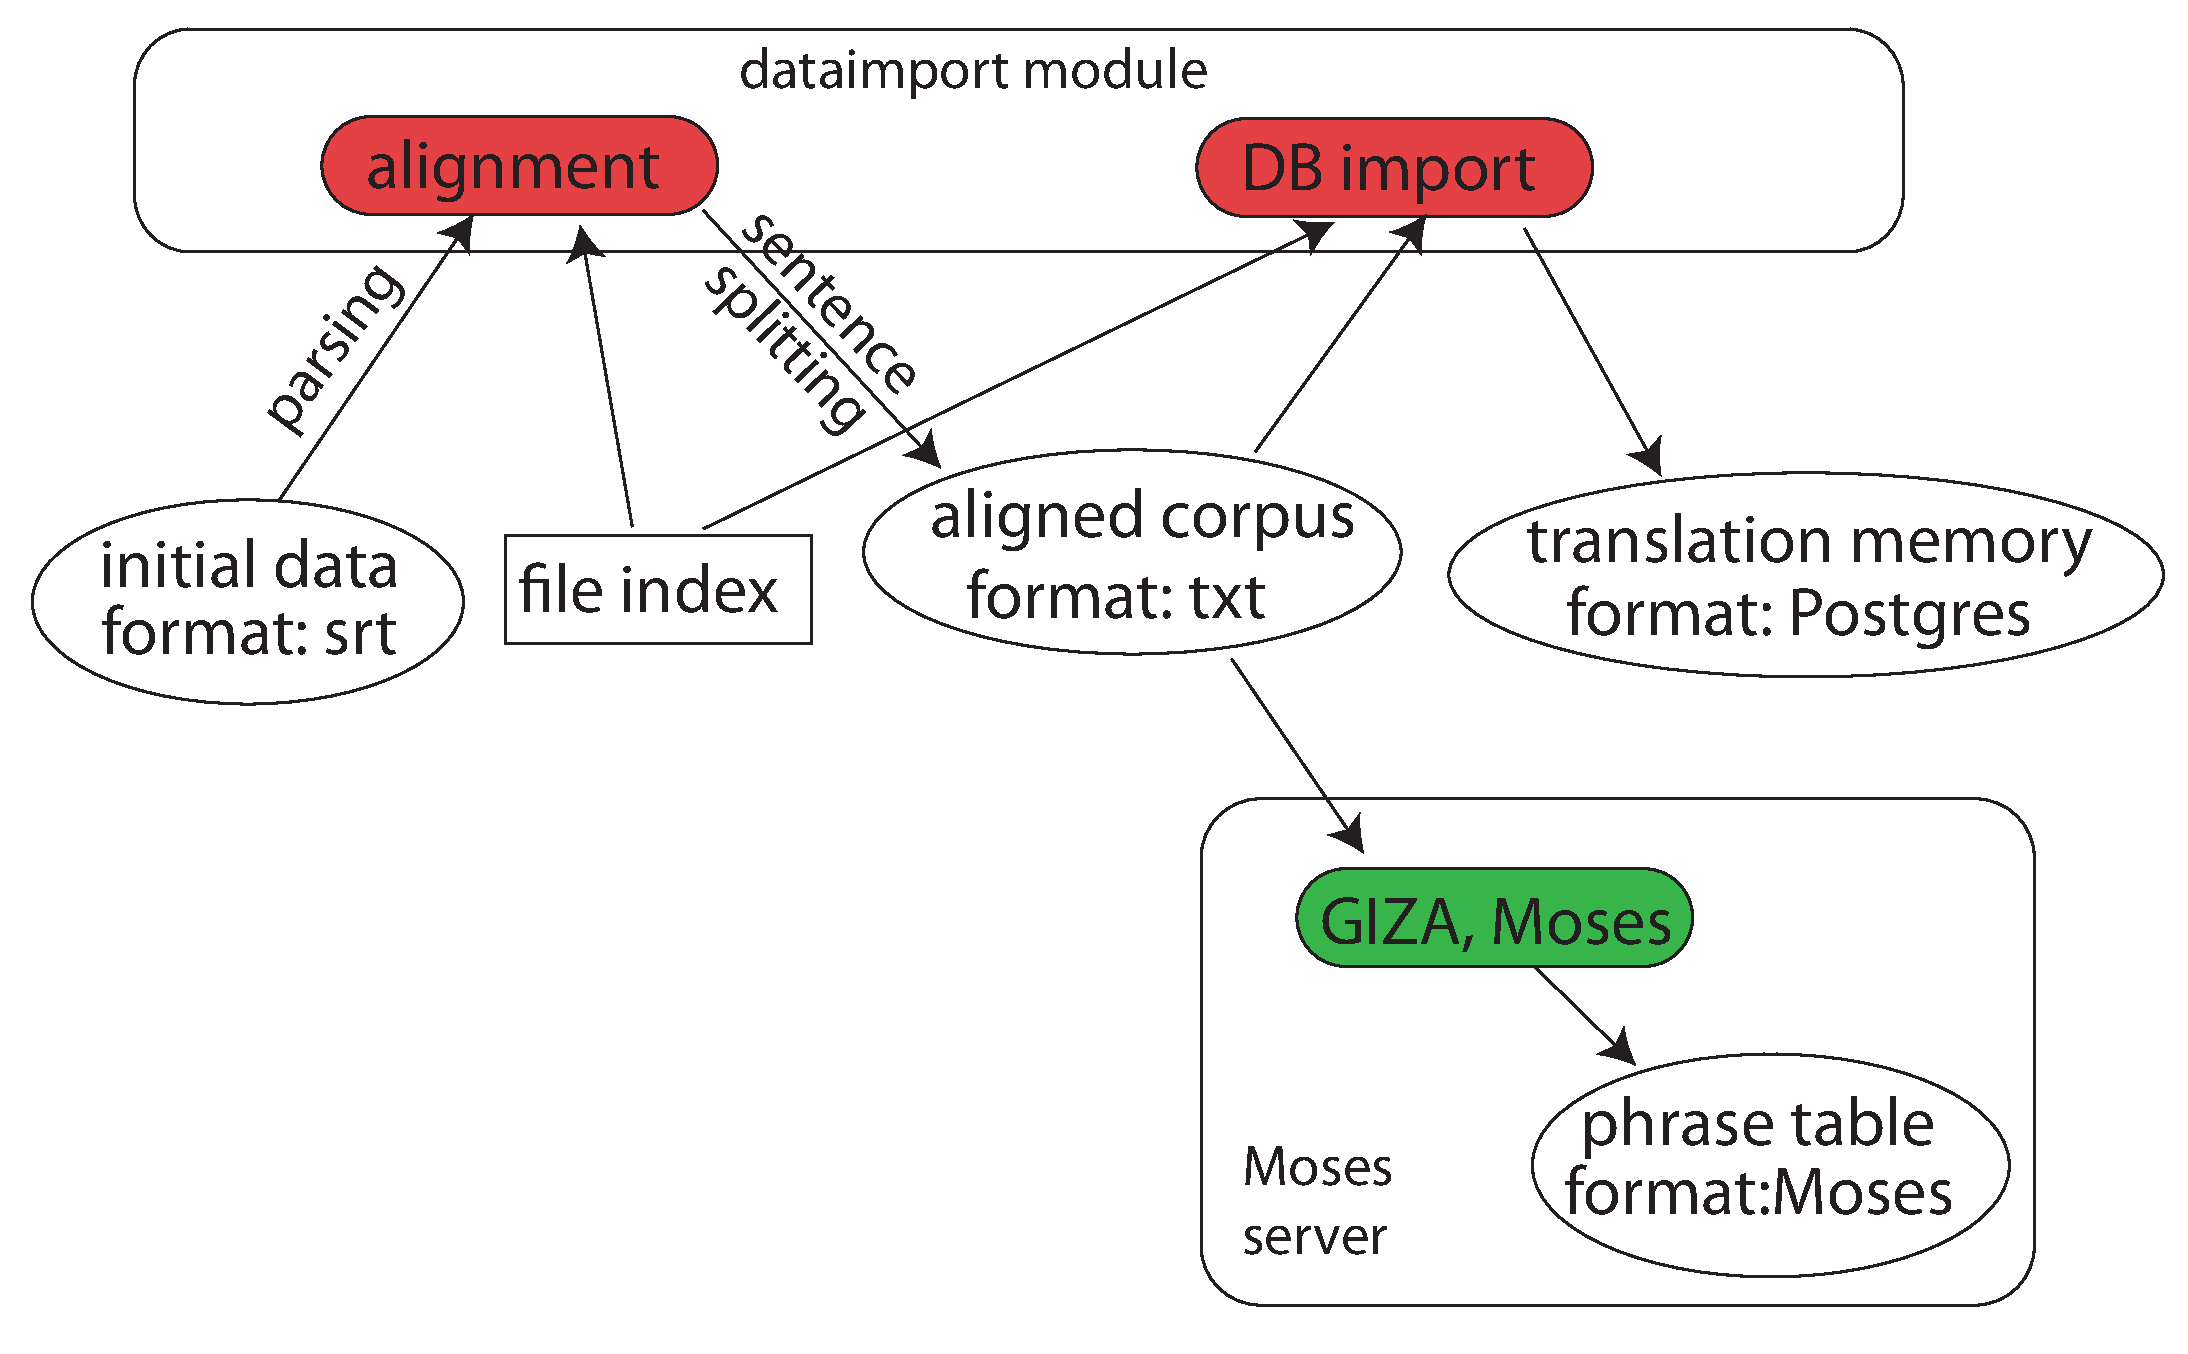
\includegraphics[width=0.8\textwidth]{figures/data_flow.pdf}
\end{center}
\caption{How do the data flow from the original archive to the database. We do not talk about the Moses server in this chapter; but it is here to illustrate that the aligned corpus is used in two ways -- in building the DB for the translation memory and in building the phrase table for MT.}\label{dataflow}
\end{figure}

\section{Loading Subtitles, Parsing}
\label{parsing_subs}
\subsection{Loading Subtitles}
The subtitles were gzipped, as already noted. Gunzipping all the files to disk would take unnecessary space, so we load the files using \texttt{GZIPInputStream}, which is a part of the standard Java library.

Most of the Czech subtitles were in \texttt{Windows-1250} encoding, but a small minority of them were in UTF-8. Some files were not in correct \texttt{gzip} format. Other than these issues, reading the files themselves was quite straightforward.

\subsection{GUI Parsing}
Before we start to talk about parsing, let us take a small sidestep to GUI.

We wanted to move the parsing of the users' uploaded subtitles to the client side. The most important reason was that we did not want to add work to the server. Therefore it was necessary to implement the parsing in the shared classes to make it available both in the GWT based GUI and the dataimport module.

This is, by the way, one of the benefits of having the dataimport module a part of the whole system. We can easily share the code with other parts of the system, and even let it be translated into JavaScript.

However, because of this, we had to write the parsing classes in such a way, that would compile with both GWT and the Java compiler. What that effectively meant was not using the standard Java Regular Expression classes, but special GWT classes.

\subsection{Parsing}
Parsing the subtitles themselves was not a hard task, using GWT's regular expression classes. Even though \texttt{sub} is considerably less popular, we decided to not neglect it and built a parser for it, too.

However, there are two scenarios, depending on when parsing is needed.

One scenario is parsing the movie subtitle after the user uploads it for translation and we want to show it to him. The second scenario is during the phase of building the corpus, where we parse the subtitles before aligning the subtitle items.

\subsubsection*{Parsing - first step}

What both scenarios have in common is the first step. In it, we take the text of the file and get only the subtitle items -- we call the subtitle item \texttt{UnprocessedChunk} and the first step \texttt{UnprocessedParser}.\footnote{As noted in the glossary, we use the word ``chunk'' in a more general sense in the source code than here in the documentation.} \texttt{UnprocessedParser} is an abstract class, that has two subclasses -- \texttt{UnprocessedParserSrt} and \texttt{UnprocessedParserSub}.

Parsing the files is a relatively straightforward task, even though we have to deal with various edge cases.

\subsubsection*{Parsing - second step}
This is where the two scenarios are different. 

When the user uploads a file, as the second step, we take those unprocessed chunks and try to split them to sentences using \texttt{TitChunkSeparator} (which, in turn, uses a \texttt{SentenceTokenizer}); we speak about sentence splitting in the next chapter. We then take those and return a list of \texttt{TimedChunk}s, with the appropriate IDs. We proceed to display the chunks using the GUI, which is not described in this chapter.

When we are building the corpus, though, we do not split the subtitle items into sentences right away. We first do alignment of files and subtitle items, which is describe below, and only then split the chunks into sentences, again using \texttt{TitChunkSeparator}.

\section{Sentence Splitting}
\label{sentence_splitting}
\subsection*{Basic idea}
Quite early on, we decided, that we should not add the whole subtitle items into the translation memory, but that we should split them to smaller parts.

As you can see on Graph~\ref{splitting:chunks}, we decided that we \emph{do} want to break subtitle items into sentences wherever possible and add those to database separately, but we do \emph{not} want to join the sentences that were already broken into multiple items.

One of the reasons for \emph{not} joining sentences together is that it is not trivial to tell if the sentence ends with a given item or not. The other reason is that the user will also have the sentences in his original subtitles split in this way. We would then, for translation, need to join his sentences in the same way - but then, we would have to break them again when exporting out again.

\begin{figure}[t]
\begin{center}
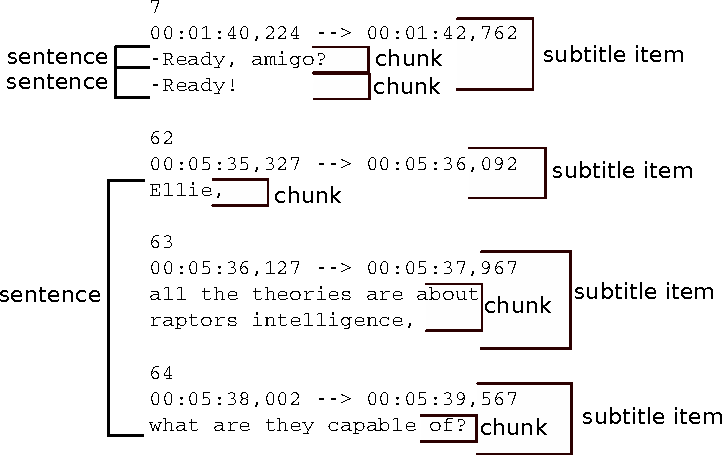
\includegraphics{figures/chunks.pdf}
\end{center}
\caption{Relation of chunk, sentence and subtitle item. From movie \emph{Jurassic Park III}}\label{splitting:chunks}
\end{figure}

To reiterate: we split sentences only within one subtitle item, and we do not join subtitle items to form complete sentences.

For the same reasons as parsing, we split sentences in the client GUI when the users upload their subtitles. That limits us in the choice of splitting algorithms, basically to just using regular expressions; any algorithms, based on some machine-learned models, are not applicable here -- we cannot link a library to the GWT code and use a model, loaded from a file.

\subsubsection*{Dialogues}
Dialogues are sometimes marked with a dash in the beginning. An example can be seen in Figure~\ref{splitting:chunks}. A dialogue is \emph{always} a new sentence.

\subsubsection*{Punctuation marks on newlines}
While punctuation marks (!?.) do not always end a sentence, they \emph{do} end a sentence when they are right before a newline character. For this reason, we do split sentences on punctuation marks before newlines.

This and the previous rule are implemented in the \texttt{TitChunkSeparator}, that is, after applying them, calling \texttt{SentenceTokenizer} for rule-based sentence splitting.

\subsubsection*{Rule-based sentence splitting}
Besides the two aforementioned rules, we use rule-based sentenced splitting (or Sentence Tokenizing) derived from code from Daniel Naber's LanguageTools.\footnote{\url{http://www.languagetool.org/}, retrieved 20.08.2012.} The code was heavily edited by us, but only for better clarity and usage of GWT regex classes, the functionality was unchanged. The code is in package \texttt{cz.filmtit.share.tokenizers}; the base class is named \texttt{SentenceTokenizer}.

The rules are, actually, not \emph{that} sophisticated; they rule out common abbreviations, names of months, cases like \texttt{I (really!) did it.}, and so on.

In the rule-based classes, the list of possible words before the punctuation that do not break the sentence have to be explicitly written in the code (because GWT has a problem with reading files). Therefore, if there was a need of adding a new language to FilmTit, this would have to be added. On the other hand, similar data are publicly available for every language in, for example, the Wiktionary project.

\section{Aligning the Subtitles}
\label{sec:aligning_subtitles}
The most crucial part in building the corpus is to group the subtitles of the same movie together.

We used two different approaches for this. Both of them need to solve these three issues:
\begin{itemize}
    \item file to file alignment -- in each movie find \emph{one} best pair
    \item filter out the ``bad'' movies -- filter out the movies, where even the best pair of file is not correctly alignable
    \item item to item alignment -- if we already have pairs of files, extract the bilingual pairs of items 
\end{itemize}

Implementation of all techniques described below are in the \texttt{cz.filmtit.dataimport.alignment} package.

\subsection{File to File Alignment}

As you could read in previous sections, we \emph{do} have some mapping from subtitles to movies. Now, we have to find out for each movie, which English and Czech file matches best together; we will throw away the rest of the files except for this one chosen pair for each movie.\footnote{Throwing away meant in the sense of building the corpus; we still have the original data, of course.}

What helps us in determining alignment is the fact, that Czech subtitles are usually created by taking existing English subtitles and translating them item by item. The timing of such files should be very similar. 

On the other hand, people, who download movies (and, therefore, subtitles) online, often use sources of questionable legality, which usually have more versions of the same file (some of them are so-called ``cam-rips'', some of them are copied from DVDs or blue-ray disks). Similarly with TV episodes -- depending on the source, the timings are slightly different. Also, in some cases, the subtitle translations are directly copied from DVD subtitles, which have totally different timing.

Sometimes, it also happens that a subtitle file has assigned a completely wrong movie tag.

To illustrate some features of the movie subtitle files, we randomly selected a movie (\emph{Legends of the Fall} from 1994) and we show fragments of \emph{all} its subtitles below. We show 5 lines from beginning, 3 lines from the middle (374 to 376, if possible), 3 lines from the end.

\label{subtitledump}

\newcommand{\nicesubs}[4]{
\noindent
\begin{boxedminipage}{\textwidth}
\begin{minipage}[b]{0.24\textwidth}\footnotesize\smaller[2]{\tt
#1
}\end{minipage}
\begin{minipage}[b]{0.24\textwidth}\footnotesize\smaller[2]{\tt
#2
}\end{minipage}
\begin{minipage}[b]{0.24\textwidth}\footnotesize\smaller[2]{\tt
#3
}\end{minipage}
\begin{minipage}[b]{0.24\textwidth}\footnotesize\smaller[2]{\tt
#4
}\end{minipage}
\end{boxedminipage}
}


\nicesubs{1 \\
00:00:00,066 \subarrow 00:00:02,375 \\
Titulky preložené do češtiny by BiGfOoT.\\
Tento disk DVD (Digital Versatile Disc)\\
je určen pouze pro domácí užití.\\
Veškerá práva k obsahové náplni včetně\\
zvukového záznamu přísluší vlastníku\\
autorského práva.\\
\\
2 \\
00:00:02,746 \subarrow 00:00:05,055 \\
Neautorizované rozmnožování, \\
úpravy, projekce pro jiné než \\
domácí \\
účely, pronájem, výměna, pújčování \\
a \\
jakákoli forma přenosu tohoto \\
disku \\
DVD nebo jeho částí jsou zakázány. \\
Porušování práv vlastníka \\
autorského\\
práva bude stíháno podle platných\\
právních předpisú.}
{
3 \\
00:00:32,666 \subarrow 00:00:38,059 \\
LEGENDA O VÁŠNI \\
\\
4\\
00:00:46,426 \subarrow 00:00:51,454\\
Někteří lidě slyší svúj\\
vnitřní hlas nadmíru jasně.\\
\\
5\\
00:00:51,626 \subarrow 00:00:54,663\\
A řídí se jím po celý život.}
{
374\\
00:56:41,186 \subarrow 00:56:44,781\\
Řekni to ještě jednou\\
a přestaneme být bratry.\\
\\
375\\
00:56:46,506 \subarrow 00:56:49,862\\
Někdy!\\
\\
376\\
00:56:52,146 \subarrow 00:56:56,503\\
- S tebou nebude šťastna.\\
- Uvidíme.}
{
755\\
02:01:42,266 \subarrow 02:01:47,101\\
... někde mezi tímto světem\\
a tím druhým.\\
\\
756\\
02:02:23,266 \subarrow 02:02:26,178\\
Byla to dobrá smrt.\\
\\
757\\
02:07:18,306 \subarrow 02:07:22,697\\
České titulky - BiGfOoT.}


\nicesubs{1 \\
00:00:00,066 \subarrow 00:00:02,375 \\
Titulky preložené do češtiny by BiGfOoT.\\
Tento disk DVD (Digital Versatile Disc)\\
je určen pouze pro domácí užití.\\
Veškerá práva k obsahové náplni včetně\\
zvukového záznamu přísluší vlastníku\\
autorského práva.\\
\\
2 \\
00:00:02,746 \subarrow 00:00:05,055 \\
Neautorizované rozmnožování, \\
úpravy, projekce pro jiné než \\
domácí \\
účely, pronájem, výměna, pújčování \\
a \\
jakákoli forma přenosu tohoto \\
disku \\
DVD nebo jeho částí jsou zakázány. \\
Porušování práv vlastníka \\
autorského\\
práva bude stíháno podle platných\\
právních předpisú.}
{
3 \\
00:00:32,666 \subarrow 00:00:38,059 \\
LEGENDA O VÁŠNI \\
\\
4\\
00:00:46,426 \subarrow 00:00:51,454\\
Někteří lidě slyší svúj\\
vnitřní hlas nadmíru jasně.\\
\\
5\\
00:00:51,626 \subarrow 00:00:54,663\\
A řídí se jím po celý život.}
{
374\\
00:56:41,186 \subarrow 00:56:44,781\\
Řekni to ještě jednou\\
a přestaneme být bratry.\\
\\
375\\
00:56:46,506 \subarrow 00:56:49,862\\
Někdy!\\
\\
376\\
00:56:52,146 \subarrow 00:56:56,503\\
- S tebou nebude šťastna.\\
- Uvidíme.}
{
755\\
02:01:42,266 \subarrow 02:01:47,101\\
... někde mezi tímto světem\\
a tím druhým.\\
\\
756\\
02:02:23,266 \subarrow 02:02:26,178\\
Byla to dobrá smrt.\\
\\
757\\
02:07:18,306 \subarrow 02:07:22,697\\
České titulky - BiGfOoT.}


\nicesubs{
1\\
00:00:46,577 \subarrow 00:00:51,605\\
Somepeople heartheir own\\
innervoices with greatcleamess.\\
\\
2\\
00:00:51,777 \subarrow 00:00:54,814\\
And they live bywhatthey hear.\\
\\
3\\
00:00:54,977 \subarrow 00:01:00,973\\
Such people become crazy,\\
orthey become legends ...}{
4\\
00:01:07,137 \subarrow 00:01:11,813\\
Tristan Ludlowwas bom\\
in the moon ofthe falling leaves.\\
\\
5\\
00:01:11,977 \subarrow 00:01:14,332\\
ltwas a terrible winter.
}{
374\\
00:56:41,337 \subarrow 00:56:44,932\\
You saythat again\\
and we're not brothers.\\
\\
375\\
00:56:46,657 \subarrow 00:56:50,013\\
Once!\\
\\
376\\
00:56:52,297 \subarrow 00:56:56,654\\
- You know you can't make her happy.\\
- l'm gonna try.
}{
756\\
02:01:38,937 \subarrow 02:01:42,247\\
He hadalways lived\\
in the borderland, anyway.\\
\\
757\\
02:01:42,417 \subarrow 02:01:47,252\\
Somewhere between this world\\
and the other.\\
\\
758\\
02:02:23,417 \subarrow 02:02:26,329\\
lt was a good death.
}


\nicesubs{1\\
00:00:58,000 \subarrow 00:01:00,696\\
- I'm here!\\
- Where? I can't see.\\
\\
2\\
00:01:02,704 \subarrow 00:01:04,365\\
I can't move!\\
\\
3\\
00:01:08,577 \subarrow 00:01:10,238\\
I'm coming!}{
4\\
00:01:35,671 \subarrow 00:01:38,037\\
I got you now.\\
\\
5\\
00:01:40,008 \subarrow 00:01:42,272\\
You're doing good.}{
315\\
00:44:59,438 \subarrow 00:45:02,032\\
were married several years ago.\\
\\
316\\
00:45:05,278 \subarrow 00:45:07,542\\
Your brother's a congressman now.\\
\\
317\\
00:45:09,282 \subarrow 00:45:11,716\\
They have a big, new place\\
in Helena.
}{}

\nicesubs{
1\\
00:00:45,869 \subarrow 00:00:49,186\\
<i>Some people hear \\
their own inner voices...</i>\\
\\
2\\
00:00:49,261 \subarrow 00:00:50,920\\
<i>with great clearness...</i>\\
\\
3\\
00:00:50,989 \subarrow 00:00:54,087\\
<i>and they live by what they hear.</i>}{
4\\
00:00:54,157 \subarrow 00:00:57,125\\
<i>Such people become crazy...</i>\\
\\
5\\
00:00:57,198 \subarrow 00:00:59,369\\
<i>or they become legends.</i>
}{
374\\
00:34:22,150 \subarrow 00:34:23,710\\
Charge!\\
\\
375\\
00:34:37,734 \subarrow 00:34:39,806\\
Goddamn it!\\
\\
376\\
00:34:40,838 \subarrow 00:34:42,693\\
- Where are you hit?\\
- It's just a scratch.
}{
983\\
02:01:38,444 \subarrow 02:01:41,891\\
<i>He had always lived\\
in the borderland anyway:</i>\\
\\
984\\
02:01:41,964 \subarrow 02:01:45,576\\
<i>somewhere between this world\\
and the other.</i>\\
\\
985\\
02:02:23,086 \subarrow 02:02:25,093\\
<i>It was a good death.</i>
}

\nicesubs{
1\\
00:00:44,411 \subarrow 00:00:47,869\\
Some people hear their own\\
inner voices\\
\\
2\\
00:00:47,948 \subarrow 00:00:49,677\\
with great clearness\\
\\
3\\
00:00:49,750 \subarrow 00:00:52,981\\
and they live\\
by what they hear}{
4\\
00:00:53,053 \subarrow 00:00:56,147\\
Such people become crazy\\
\\
5\\
00:00:56,223 \subarrow 00:00:58,487\\
or they become legend
}{
374\\
00:35:27,326 \subarrow 00:35:30,921\\
Is that wrong to want\\
to distinguish myself gloriously\\
\\
375\\
00:35:30,996 \subarrow 00:35:33,226\\
in combat as my father did?\\
\\
376\\
00:35:33,298 \subarrow 00:35:36,290\\
Tristan and Alfred\\
watch over me so carefully
}{
1000\\
02:06:50,103 \subarrow 02:06:53,869\\
Somewhere between this world\\
and the other\\
\\
1001\\
02:07:32,979 \subarrow 02:07:35,072\\
It was a good death\\
\\
1002\\
02:12:47,200 \subarrow 02:12:49,072\\
\{\{\{the end\}\}\}
}


\nicesubs{
1\\
00:00:43,411 \subarrow 00:00:46,869\\
Some people hear their own\\
inner voices\\
\\
2\\
00:00:46,948 \subarrow 00:00:48,677\\
with great clearness\\
\\
3\\
00:00:48,750 \subarrow 00:00:51,981\\
and they live\\
by what they hear}{
4\\
00:00:52,053 \subarrow 00:00:55,147\\
Such people become crazy\\
\\
5\\
00:00:55,223 \subarrow 00:00:57,487\\
or they become legend
}{
374\\
00:35:26,326 \subarrow 00:35:29,921\\
Is that wrong to want\\
to distinguish myself gloriously\\
\\
375\\
00:35:29,996 \subarrow 00:35:32,226\\
in combat as my father did?\\
\\
376\\
00:35:32,298 \subarrow 00:35:35,290\\
Tristan and Alfred\\
watch over me so carefully
}{
1000\\
02:06:49,103 \subarrow 02:06:52,869\\
Somewhere between this world\\
and the other\\
\\
1001\\
02:07:31,979 \subarrow 02:07:34,072\\
It was a good death\\
\\
1002\\
02:12:46,200 \subarrow 02:12:48,072\\
\{\{\{the end\}\}\}
}

\nicesubs{
1\\
00:00:46,418 \subarrow 00:00:51,446\\
Some people hear their own\\
inner voices with great clearness.\\
\\
2\\
00:00:51,618 \subarrow 00:00:54,655\\
And they live by what they hear.\\
\\
3\\
00:00:54,818 \subarrow 00:01:00,814\\
Such people become crazy,\\
or they become legends ...}{
4\\
00:01:06,978 \subarrow 00:01:11,654\\
Ôristan Ludlow was born\\
in the moon of the falling leaves.\\
\\
5\\
00:01:11,818 \subarrow 00:01:14,173\\
It was a terrible winter.
}{
374\\
00:56:58,898 \subarrow 00:57:02,208\\
You will fail.\\
\\
375\\
00:57:14,298 \subarrow 00:57:17,529\\
I'm going to be leaving today.\\
\\
376\\
00:57:26,458 \subarrow 00:57:30,087\\
l do wish you both all the best.
}{
752\\
02:01:42,258 \subarrow 02:01:47,093\\
Somewhere between this world\\
and the other.\\
\\
753\\
02:02:23,258 \subarrow 02:02:26,170\\
It was a good death.\\
\\
754\\
02:07:18,298 \subarrow 02:07:22,689\\
English subtitles - lFT
}

\nicesubs{
1\\
00:00:45,977 \subarrow 00:00:51,005\\
Some people hear their own\\
inner voices with great cleamess.\\
\\
2\\
00:00:51,177 \subarrow 00:00:54,214\\
And they live by what they hear.\\
\\
3\\
00:00:54,377 \subarrow 00:01:00,373\\
Such people become crazy,\\
or they become legends ...}{
4\\
00:01:06,537 \subarrow 00:01:11,213\\
Tristan Ludlow was bom\\
in the moon of the falling leaves.\\
\\
5\\
00:01:11,377 \subarrow 00:01:13,732\\
lt was a terrible winter.
}{
374\\
00:56:40,737 \subarrow 00:56:44,332\\
You saythat again\\
and we're not brothers.\\
\\
375\\
00:56:46,057 \subarrow 00:56:49,413\\
Once!\\
\\
376\\
00:56:51,697 \subarrow 00:56:56,054\\
- You know you can't make her happy.\\
- l'm gonna try.
}{
756\\
02:01:38,337 \subarrow 02:01:41,647\\
He had always lived\\
in the borderland, anyway.\\
\\
757\\
02:01:41,817 \subarrow 02:01:46,652\\
Somewhere between this world\\
and the other.\\
\\
758\\
02:02:22,817 \subarrow 02:02:25,729\\
lt was a good death.
}

\nicesubs{
1\\
00:00:43,785 \subarrow 00:00:47,243\\
Some people hear their own\\
inner voices...\\
\\
2\\
00:00:47,322 \subarrow 00:00:49,051\\
with great clearness...\\
\\
3\\
00:00:49,123 \subarrow 00:00:52,354\\
and they live\\
by what they hear.
}{
4\\
00:00:52,427 \subarrow 00:00:55,521\\
Such people become crazy...\\
\\
5\\
00:00:55,597 \subarrow 00:00:57,861\\
or they become legends.
}{
374\\
00:35:35,741 \subarrow 00:35:37,470\\
I may never get the opportunity.\\
\\
375\\
00:35:46,085 \subarrow 00:35:47,712\\
Charge!\\
\\
376\\
00:36:02,334 \subarrow 00:36:04,495\\
Goddamn it!
}{
987\\
02:06:45,772 \subarrow 02:06:49,367\\
He had always lived\\
in the borderland anyway:\\
\\
988\\
02:06:49,443 \subarrow 02:06:53,209\\
somewhere between this world\\
and the other.\\
\\
989\\
02:07:32,319 \subarrow 02:07:34,412\\
It was a good death.
}

As can be seen, the two Czech subtitle files are exact copies of each other. Also, there is one English subtitle that is totally wrong. Except for this one, most of the English files seems to match the Czech one quite well. None of them is a ``perfect'' match, looking either at numbers or at the timing. Judging by the \emph{number} of the last translation -- some are from a similar source (those with around 750 chunks), while those with significantly more chunks are probably from different source. Although, there is no perfect match, there are few almost-perfect matches.

On average, there is 2.1 Czech subtitle files and 5 English subtitle files per movie. However, the numbers are not evenly distributed and very popular movies can have tens of subtitles.

If we take for \emph{each} movie \emph{all} the pairs, where Czech is one side and English on the other (but both have the same movie), we have 235.825 such pairs (reminding, we originally had 139.538 files).

\subsection{Subtitle to Subtitle Alignment}
As written above, translations of subtitles are usually done directly from other subtitles, so the alignment is entirely based on time marks. We do \emph{not} look at any other features.\footnote{In \emph{Using Movie Subtitles for Creating a Large-Scale Bilingual Corpora (Einav Itamar, Alon Itai)}, authors tried to use other features, but we used just the time info.}

However, even in the cases when a Czech subtitle file has been made directly from an English one, there are still cases where, for example, one chunk is split into two chunks, two are merged into one and so on. Sometimes, the English version of the subtitles is done for people with hearing impairment and, therefore, describes all the sounds, while the Czech version has those deleted.

The result of this step is a list of pairs of the Czech and English subtitle items. We do this step only on the chosen pair of files from the previous step, and only if the pair of the files is chosen as a ``good'' candidate.

After this step, we almost have the final corpus. What we have to do before saving it into a final corpus is splitting the aligned items into chunks, as described in Section~\ref{sentence_splitting}. If both Czech and English have the same number of chunks, we split them and add those to the corpus; if the number is different, we ignore them.


\subsection{Approaches}
\subsubsection{Equality with tolerance}

\begin{figure}[t]
\begin{center}
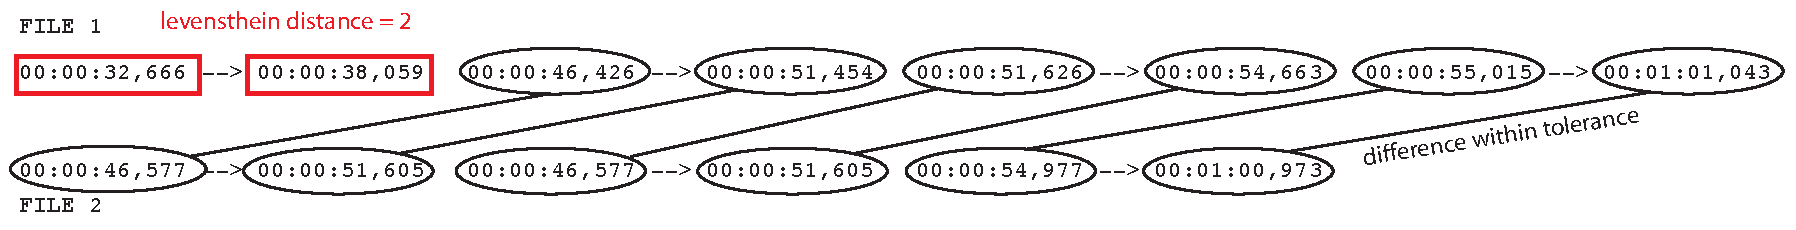
\includegraphics[width=\textwidth]{figures/tolerance_priklad.pdf}
\end{center}
\caption{Levenshtein distance for file-to-file alignment}\label{tolerance}
\end{figure}

The first approach is to take only the items with the same time as belonging to each other.

However, the times are rarely exactly equal. One of the paper authors\footnote{Einav Itamar, Alon Itai (2008): \emph{Using Movie Subtitles for Creating a Large-Scale Bilingual Corpora.} The sixth international conference on Language Resources and Evaluation, LREC 2008.} used 0.6\,s as a tolerance in order not to be confused by slight differences in timing.

We observed that if we use a bigger tolerance, we have more subtitle pairs, but sometimes with worse quality (because sometimes we get totally different subtitles, not belonging to each other). We tried tolerance 0.6\,s (as suggested by the paper), and then 6\,s.

For counting file to file alignment, we count editing distance of their time marks, as illustrated in Figure~\ref{tolerance}; we use a dynamic algorithm for that.

We take all the time information (both the starts and the ends) as vectors. Then, we count editing distance of those two vectors, where we take the two time informations as equal if they fall within tolerance, otherwise we take them as unequal. We score all possible pairs of Czech subtitle files on one side and English on the other for the given movie and we use the Levensthein distance as a score; the file pair with the shortest Levensthein distance is the ``chosen'' file pair.

We use Levensthein distance because there can be some small splitting, additions, and so on, but we want to take the pair of files, that have minimal number of these.

For filtering out the ``bad'' movie pairs, we just throw away all that has editing distance higher than 30. (This was decided empirically by looking at some random subtitle files.)

For subtitle to subtitle alignment, we take the subtitles that have a distance of both beginning and ending within the tolerance. Because the computation on the whole files would be very time consuming, we limited it to just the first 100 time marks in the files.


%deleting this, since I covered it in previous section already
%While comparing two mostly identical subtitle files, there may appear some issues which cause that the timing of the files is not identical. There exist some cases where one chunk is split into more or two are merged into one. In both of this cases, two time declarations in the file remain the same and two time declarations are added or deleted. There are also a lot of subtitles for deaf people where from time to time some additional subtitle appears. 
%From that we concluded that the best measure how subtitle files matches would be the editing distance of their time declarations since the cases mentioned above contributes relatively little to the score in contrast to some more significant mismatches. 
%By that we mean taking all the time information (both the starts and the ends) as vectors, and then counting editing distance of those two vectors by dynamic algorithm.
%As one of the papers (CITE!!!) proposed we used 0.6\,s as a tolerance for equality, not to be confused by slight differences in timing. Because the computation on whole files would be really time consuming, we limited it just for the first 100 time declarations in the files.

\begin{figure}[t]
\begin{center}
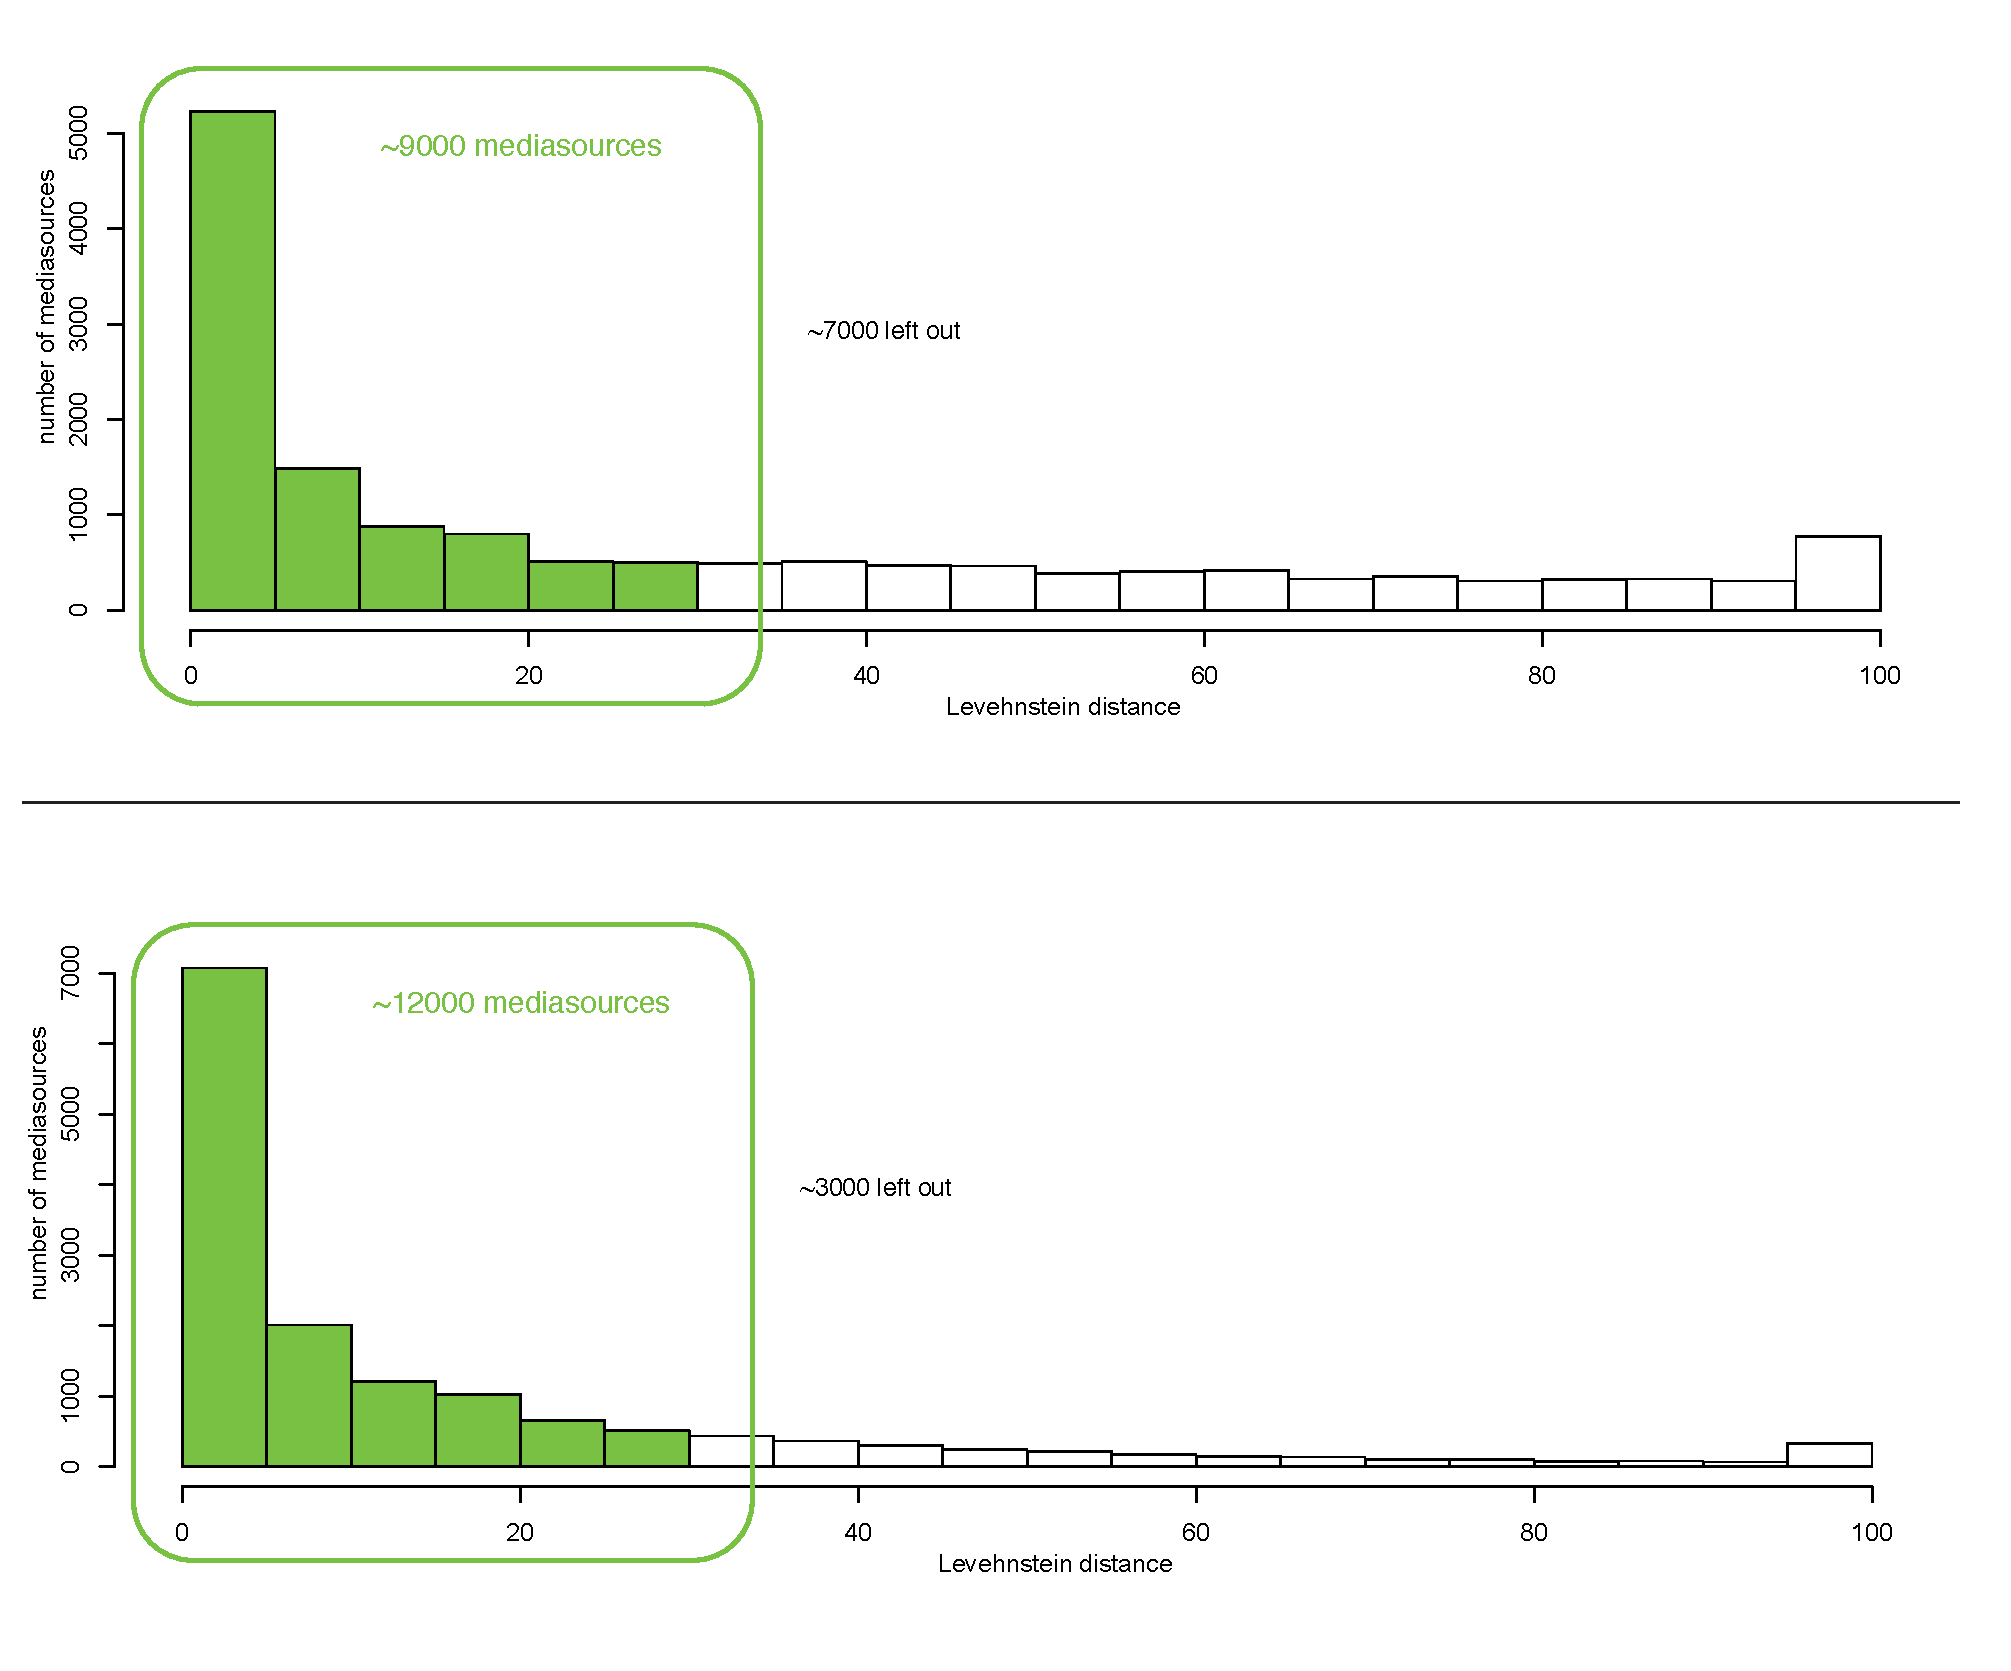
\includegraphics[width=\textwidth]{figures/histograms.pdf}
\end{center}
\caption{Levenshtein distances for 0,6s tolerance (above) and 6s tolerance (below)}\label{histograms}
\end{figure}

You can see the histogram of shortest Levensthein distances for each movie in Figure~\ref{histograms}. The green part represents the ``good'' file pairs. The distance is maximally 100, since we take only the first 100 subtitles from each file. You can already see that there are more files in the bigger tolerance. (Of course, they might be also more wrong.)


%This whole thing doesn't make much sense to me, at all (how are those percents computed? why are those in percent when we use levenstein distance? or is this the sub-to-sub alignment? is it percentage of what exactly? It doesn't make much sense to me)
%I am commenting it all
%The results were following: from 15,552 movies there was 22.2\,\%
%with perfect matches and 3.1\,\% of total mismatches. The scores for partial matches are captured in table \ref{opensubtitles:matchTable}.
%\begin{table}[h]
%
%\begin{center}
%\begin{tabular}{|c|c|}
%\hline
%amount of films & measure of match\\ \hline
%22,2 \% & $= 100 \%$ match \\
%45.7 \% & $\ge 90 \%$ match \\ 
%56.2 \% & $\ge 80 \%$ match \\ 
%63.0 \% & $\ge 70 \%$ match \\
%69.2 \% & $\ge 60 \%$ match \\ \hline
%\end{tabular}
%\end{center}
%
%\caption{Table capturing for how many movies there exist a matching pair of subtitle files with given measure of matching as a percentage of timings which do not contribute to editing distance (in other words percentage of timings which are with the given tolerance equal in both files).}\label{opensubtitles:matchTable}
%\end{table}
%After looking at some randomly selected files we have decided to use just movies for which we have a pair of files where at least 70\,\% of timings match. Again, lower match score doesn't mean lower quality of translation, but rather how the subtitles match to each other. 

The chunk-to-chunk alignment is then simple -- chunks are aligned together if both the time of their start and time of their end differ less than by the tolerance.

%This gave us 884 MB of parallel data which consists of 13,636,022 chunks. In this we have 5,669,837 unique chunks, from which 3.7 \% appears more than once. On the other hand, chunks appearing more than once make 57.6 \% of the whole corpus.
%I will add the sizes of the various corpora to the evaluation, it will make more sense anyway

\subsubsection{Shortest distance}
\begin{figure}[t]
\begin{center}
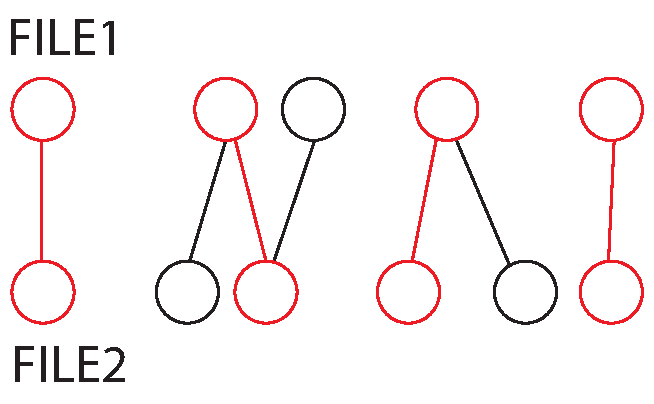
\includegraphics[width=0.5\textwidth]{figures/distance_align.pdf}
\end{center}
\caption{An illustration for the distance-based alignment. Circle represents subtitle, red line represent chosen alignment, black ones are some candidates, red circles are the subtitles that are aligned}\label{histograms}
\end{figure}

The idea that lead to the next approach was -- what if we didn't have any maximal tolerance and just took the subtitles that are closest to each other.

More concretely, we took the middle time of each chunk (in milliseconds) and counted distance from other chunk as an absolute difference of these middles. 

To find the best matching pairs in pair of two files, we took the closest Czech chunk for each English chunk; then, if more English chunks were aligned with the same Czech chunks, we select the closest.

(Although similar, this is not a case of graph matching in bipartite graphs, since it is \emph{not} needed that each Czech chunk would have some English chunk and vice versa.)

Trivially implemented this algorithm would be quadratic to the size of subtitle file; however, we may dynamize it so even the worst case has linear time to the size of the subtitle file.

In the file-to-file alignment case, we count this alignment for each pair of files and then we sum all the distances for a given pair of files; we then select the pair with the smallest sum as the correct one. If the subtitles are just translated from each other, the sum should be small and can be even zero, if the time marks are exactly the same.

We then selected given number of movies (we tried 6,000 and 12,000) with the smallest sum as the ``good'' movie pairs and then align them.

\subsubsection{Baseline -- trivial alignment}
As a baseline for comparison, the ``trivial'' algorithm just takes first filepair that it sees for a given movie, then takes all the movies, and then aligns first chunk on source side with first chunk on target side, second with the second one and so on.

\subsection{Evaluation of Alignments}
We have two slightly different approaches to counting the alignment of subtitles. The question is, which one to choose. For having a more rigorous evaluation than just manual comparing of random files it was necessary to develop a metric which captures the quality of the alignment which is described later.

\subsubsection{Size of corpus}
One of the most simple evaluations is just the sheer size. Since the alignment classes are modular, we can actually use different file-to-file alignment together with subtitle-to-subtitle alignment.

\begin{table}[h]
\begin{center}
\begin{tabular}{|l|l|r|}
    \hline
    \textbf{file alignment} & \textbf{subtitle alignment} & \textbf{number of pairs} \\ \hline
    Tolerance 0,6 s & Tolerance 0,6 s & 5.412.875 \\ \hline
    Tolerance 6 s & Tolerance 0,6 s & 7.210.505 \\  \hline
    Tolerance 6 s & Tolerance 6 s & 9.228.304 \\ \hline
    Tolerance 6 s & Distance & 4.660.382 \\ \hline
    Distance 6.000 & Distance & 2.109.017 \\ \hline
    Distance 12.000 & Distance & 4.177.117 \\ \hline
    Distance 6.000 & Tolerance 6s & 4.024.876 \\ \hline
    Distance 12.000 & Tolerance 6s & 7.982.142 \\ \hline
    Trivial & Trivial & 8.318.225 \\ \hline
    
\end{tabular}
\end{center}

\caption{Size of corpus}\label{corpusize}
\end{table}

As can be seen in Table~\ref{corpusize}, the highest tolerance produces the biggest corpus, while Distance-based alignment does not produce as much.

What is interesting is that the Trivial alignment -- that really takes \emph{everything} -- has smaller corpus than the one with the higher tolerance.


\subsubsection{Manual alignment}
Another measurement is to compare the alignment with a human alignment.

What is sometimes proposed in cases on alignment evaluation is letting users align something and then measure that against the aligner output.

The problem is -- what to manually align exactly in our case? We can manually align \emph{files} for a given movie (we have shown an example of all files for a movie in \ref{subtitledump}). It is not very easy though, since -- as we have seen already -- the files are all \emph{more or less} correct translations and the timings are not exact matches. Nonetheless, we randomly selected 30 movies and for each of these, selected which pairs of \emph{files} seems like from the same source and match together.

However, there is a bigger issue with the manual chunk-to-chunk alignment, that is -- which file pairs to manually align? Since we do not know the file-to-file aligner's results in advance, we should align all the file pairs -- but if there are, for example, 10 subtitle files on each language, it produces hundreds of pairs of files on which we should provide manual alignment, while the texts in all of them are \emph{mostly} the same, but \emph{not exactly} the same. This actually proved too hard and tedious to do.

Moreover, the aligner chooses just one pair, but a person would have to align all the possible pairs for no reason (a person can also produce different errors in different file pairs, which could be ``unfair'' to some of the aligners).

Therefore, we manually annotated just the file-to-file alignment and we tried a different metric on the whole chunk-to-chunk alignment.

\subsubsection{Counting precision and recall for file to file alignment}
There are five cases of possible events:

\begin{itemize}
    \item With manual alignment, we found no possible matches and the aligner did not mark it as a ``good'' movie - in this section, we call this \textit{true negative}
    \item With manual alignment, we found possible matches, but the aligner did not mark it as a ``good'' movie - in this section, we call this \textit{false negative}
    \item With manual alignment, we found no possible matches, the aligner marked it as a ``good'' movie and included it in corpus - in this section, we call this \textit{false positive}
    \item With manual alignment, we found possible matches, the aligner marked it as a ``good'' movie, but the match from aligner was not one of the correct ones -  we call this \textit{partly true positive}
    \item  With manual alignment, we found possible matches, the aligner marked it as a ``good'' movie and the match from aligner was  one of the correct ones -  we call this \textit{fully true positive}
\end{itemize}

With some consideration, we count precision as \footnote{Strictly speaking, it is not precision or recall. However, intuitively it captures similar qualities and it may be more confusing to use a different terminology.}

$$\frac{\text{fully true positive}}{\text{false positive}+\text{fully true positive}+\text{partly true positive}},$$ and recall as $$\frac{\text{fully true positive}}{\text{fully true positive}+\text{partly true positive}+\text{false negative}}.$$

This means precision is the percentage of movies chosen by the aligner that are aligned correctly; recall is the percentage of movies that \emph{can} be aligned (from manual alignment), that are aligned correctly. Results for the algorithms are in Table~\ref{align_score}.

\begin{table}[h]
\begin{center}
\begin{tabular}{|l|c|c|c|} 
    \hline
    \textbf{approach} & \textbf{precision} & \textbf{recall} & \textbf{F1-measure} \\ \hline
    Baseline & 33 & 33 & 33 \\ \hline
    Tolerance 6s & 61 & 57 & 59 \\ \hline
    6,000 best distance-based & 67 & 20 & 31 \\ \hline
    12,000 best distance-based & 76 & 53 & 63 \\ \hline
\end{tabular}
\end{center}

\caption{Performance of the alignment algorithms (as percentage)}\label{align_score}
\end{table}

\subsubsection{Simulation of translation memory}
We tried a different evaluation metric for testing the alignments.

We imported the whole corpus (as created by an aligner) except for 30 randomly selected media sources into a database, then we took 20 chunks from each of the 30 files and queried it to a translation memory. We looked at the result this translation memory has given us and judged how much of it was relevant.

We did not test it on the real database (since building it multiple times would be too time consuming), we searched just for direct matches using standard Java\footnote{Standard Java, but it's in Scala} ``equals''.

\subsubsection{Translation memory simulation result}

We counted two percentages for each configuration -- the one we called \emph{precision} -- that is, how many of the received translation results were correct -- and the second that we called \emph{coverage} -- that is, \emph{how many of the subtitle chunks received at least one good translation}.

We also calculated a harmonized mean of those two.

What also has to be noted here is that the result counts are not evenly distributed -- for the more frequent sentences like ``I don't know'', we might have hundreds of matches; we receive only the first 30 matches. This will, of course, skew the precision slightly (since we take only 30 chunks as received); however, it still emulates the working of translation memory.

Results of the experiment are tabulated in \ref{tm_simulation}.

\begin{table}[h]
\begin{center}
\begin{tabular}{|l|l|r|r|r|}
    \hline
    \textbf{file alignment} & \textbf{subtitle alignment} & \textbf{precision} & \textbf{coverage} & \textbf{mean} \\ \hline
    Tolerance 0,6 s & Tolerance 0,6 s & 96  & 19  & 31 \\ \hline
    Tolerance 6 s & Tolerance 6 s & 82  & 29 & 43 \\ \hline
    Tolerance 6 s & Distance & 83 & 24 & 37 \\ \hline
    Distance 6.000 & Distance &  89 & 21 & 35 \\ \hline
    Distance 12.000 & Distance & 85 & 24 & 38 \\ \hline
    Distance 6.000 & Tolerance 6s & 79 & 24 & 36 \\ \hline
    Distance 12.000 & Tolerance 6s & 78 & 27 & 41 \\ \hline
    Trivial & Trivial & 15 & 20 & 17 \\ \hline
    
\end{tabular}
\end{center}

\caption{Size of corpus}\label{tm_simulation}
\end{table}

It can be noticed that the Distance is always worse than Tolerance. Also, we might notice, that every time we somehow allowed more files, the precision went down, but the coverage went up.

The baseline algorithm is absurdly tolerant and produces actually bigger coverage than the tolerance-based algorithm with tolerance 600 ms. However, the precision is very low.

Also note that even with the alignment with best coverage, we still covered only slightly more than one fourth of the file. We see that we really \emph{need to} use fuzzy matching and, if possible, machine translation, both of which we use in the final software.

We chose the tolerance-based algorithm with 6s tolerance, since it has the best harmonic mean and mainly has the biggest coverage with still relatively precise translations. Users of Machine Translation can easily ignore a possible wrong translation, if they do not like it.

\section{Running the Alignment}
The alignment can also be re-run. The needed Scala objects with appropriate \texttt{main} methods are in \texttt{cz.filmtit.dataimport.alignment.tasks} package. However, it is has not been tested on any other data than our data. The locations of the initial data, the \texttt{export.txt} file and the directory where the corpus will be located has to be set in \texttt{configuration.xml}.

Alignment with any of the methods takes about 4 hours on a Linux PC with Intel Core2 Quad CPU with 2.83GHz with 4GB of memory.

Also, the tests that produced the results in this section are in the same package. However, as they were intended to be run only once, they may have paths and options hardcoded in the source code.
